% -*- coding: utf-8; -*-

\chapter{Mapeamento do Volume}

No presente capítulo é apresentado o mapeamento da movimentação das seções no volume. A movimentação das seções em cada \emph{EtapaMS} de restauração acabará por determinar uma movimentação do volume. Tendo em vista que as superfícies do modelo foram mapeadas como apresentado anteriormente, a movimentação dessas superfícies também é mapeada no volume. 

Este mapeamento do volume tem o intuito de fornecer uma maneira de realizar o acompanhamento de pontos dispostos no domínio tridimensional do modelo geológico durante o processo de restauração. Com isso, é possível obter mais informações sobre o que ocorre fora das seções e superfícies geológicas.

Neste capítulo são apresentadas a metodologia para o mapeamento do volume e sua aplicação dentro do Sistema Recon, bem como detalhes sobre os requisitos para utilização do método. Uma breve discussão sobre a metodologia de mapeamento do volume também é descrita neste capítulo. A implementação computacional dessa metodologia foi realizada na biblioteca \emph{MGeo Deformer} por Müller~\cite{Muller}.

\section{Metodologia}\label{vol-metodology}

Nas últimas décadas vários métodos numéricos vêm sendo desenvolvidos para simulação de problemas físicos em modelos tridimensionais, dentre os quais destacam-se alguns, divididos em dois grupos e listados a seguir:

\renewcommand{\labelitemi}{•}
\begin{itemize}
  \item Métodos baseados em malhas tridimensionais: métodos de elementos finitos (FEM)\cite{MEF}; métodos de diferenças finitas (FDM)\cite{MDF}; métodos de volumes finitos (FVM)\cite{MVF}; métodos lagrangeanos euleriano arbitrário (ALE)\cite{ALE}.
  \item Métodos não baseados em malhas tridimensionais: método de partículas em células (PIC)\cite{PIC}; smooth particle hydrodynamics (SPH)\cite{SPH}; método de ponto material (MPM)\cite{MPM}; método de elementos discretos (DEM)\cite{DEM}; método de ponto material com interpolação generalizada (GIMP)\cite{GIMP,MullerGIMP}.
\end{itemize}

De maneira genérica, o problema físico-matemático para o mapeamento do volume baseado em restauração de seções e mapeamento de superfícies pode ser descrito por: dada a movimentação de um conjunto de seções e a movimentação de um conjunto de superfícies, movimentar um volume de forma compatível, respeitando restrições de movimentação nas falhas. Todos os métodos acima citados, além de outros não referenciados nesta lista, apresentam vantagens e desvantagens e poderiam ser utilizados para solucionar este problema. Todavia, a escolha de um método numérico deve contemplar as características do problema que por vezes demanda simplificações e/ou aprimoramentos além da avaliação da viabilidade de uso, por exemplo: tempo para simulação, geração de dados de entrada, estabilidade numérica, entre outros. De forma geral, modelos geológicos tridimensionais apresentam características de grande complexidade geométrica. Essa complexidade, por sua vez, acarreta grandes desafios para geração de malhas, especialmente quando devem ser consideradas restrições de horizontes e falhas. Além disso, de forma geral em Geologia, as etapas de modelagem e simulação tridimensionais apresentam soluções caras computacionalmente. Tendo em vista estes aspectos, Muller~\cite{Muller} desenvolveu uma metodologia de solução do problema matemático exposto anteriormente, baseada principalmente nos métodos GIMP e ALE, apresentada a seguir.

O problema físico-matemático é caracterizado pela movimentação do volume, que por sua vez é guiado pela movimentação de seções transversais e/ou superfícies. Dessa forma, as equações de conservação de massa e conservação de momento são suficientes para a solução do problema, Eqs.~\ref{eq-vol-1} e~\ref{eq-vol-2} respectivamente. Na conservação de momento, devido às características do problema, o termo relativo às forças de corpo (gravitacionais) pode ser desconsiderado.

\begin{align}
  &\frac{d\rho}{dt} + \rho \mathbf{\nabla}\cdot\boldsymbol{v} = 0\label{eq-vol-1}
\end{align}

\begin{align}
  &\rho\frac{d\boldsymbol{v}}{dt} - \mathbf{\nabla} \cdot \boldsymbol{\sigma} = 0\label{eq-vol-2}
\end{align}

Nas equações acima $\rho$ representa densidade, $\boldsymbol{v}$ velocidade e $\boldsymbol{\sigma}$ o tensor de tensões de Cauchy. Para evitar a necessidade de geração de malhas tridimensionais, a solução das Eqs.~\ref{eq-vol-1} e~\ref{eq-vol-2} será desenvolvida para um meio representado por pontos discretos arbitrários, em suas coordenadas $\boldsymbol{x}_p$, que por sua vez representam o volume $\Omega$ do modelo. A conectividade entre esses pontos será dada por uma grade volumétrica, em suas coordenadas $\boldsymbol{x}_i$.

A massa de cada ponto arbitrário pode ser descrita por:

\begin{align}
  &m_p =\int_{\Omega}\rho(\boldsymbol{x}_p)\chi(\boldsymbol{x}_p)\,d\Omega.
\end{align}

Sendo $\rho(\boldsymbol{x}_p)$ o campo de densidades e $\chi(\boldsymbol{x}_p)$ funções características. Para caracterizar a ligação entre os pontos e a grade são utilizadas funções peso $\boldsymbol{N}_{ip}$. Uma função $\boldsymbol{N}_{ip}$ representa o peso para o nó $i$ da grade avaliado na posição do ponto $p$, $\boldsymbol{N}_{ip} = \boldsymbol{N}(\boldsymbol{x}_p-\boldsymbol{x}_i)$ definido por:

\begin{align}
  &\boldsymbol{N}_{ip} = \frac{\displaystyle\int_{\Omega}\chi(\boldsymbol{x})\boldsymbol{\Phi}_i(\boldsymbol{x})\,d\Omega}{\displaystyle\int_{\Omega}\chi(\boldsymbol{x})\,d\Omega}.
\end{align}

Onde $\boldsymbol{\Phi}_i(\boldsymbol{x})$ é uma função de forma para o nó $i$. O gradiente da função peso pode ser definido por:

\begin{align}
  &\nabla\boldsymbol{N}_{ip} = \frac{\displaystyle\int_{\Omega}\chi(\boldsymbol{x})\nabla\boldsymbol{\Phi}_i(\boldsymbol{x})\,d\Omega}{\displaystyle\int_{\Omega}\chi(\boldsymbol{x})\,d\Omega}.
\end{align}

As funções características e de forma utilizadas na presente formulação são:

\begin{align}
  &\chi(\boldsymbol{x_p}) = 
    \begin{cases}
      1 &\text{se } |\boldsymbol{x_p}| < \cfrac{l}{2}\\
      0 &\text{em outro caso}
    \end{cases}\label{eq-vol-carac-1}
\end{align}

\makeatletter
\NewDocumentCommand{\eqmathbox}{o O{c} m}{%
  \IfValueTF{#1}
    {\def\eqmathbox@##1##2{\eqmakebox[#1][#2]{$##1##2$}}}
    {\def\eqmathbox@##1##2{\eqmakebox{$##1##2$}}}
  \mathpalette\eqmathbox@{#3}
}
\makeatother

\begin{align}
  &\Phi(\boldsymbol{x_p}) = 
    \begin{cases}
      \eqmathbox[eqn1]{1 - \cfrac{4\boldsymbol{x_p}^2+l}{4hl}} & \text{ se } |\boldsymbol{x_p}| < \cfrac{l}{2}\\
      \\
      \eqmathbox[eqn1]{1 - \cfrac{|\boldsymbol{x_p}|}{h}} & \text{ se } \cfrac{l}{2} \leqslant |\boldsymbol{x_p}| < h - \cfrac{l}{2}\\
      \\
      \eqmathbox[eqn1]{\cfrac{\left(h+\cfrac{l}{2}-|\boldsymbol{x_p}|\right)^2}{2hl}} & \text{ se } h-\cfrac{l}{2} \leqslant |\boldsymbol{x_p}| < h + \cfrac{l}{2}\\
      \\
      \eqmathbox[eqn1]{0} & \text{ em outro caso}
    \end{cases}\label{eq-vol-carac-2}
\end{align}

Nas Eqs.~\ref{eq-vol-carac-1} e~\ref{eq-vol-carac-2}, $h$ representa o tamanho da célula da grade e $l$ um tamanho característico definido inicialmente em função do número de pontos contidos na célula.

Como já mencionado, o volume é representado por pontos arbitrários. De forma semelhante, as seções e superfícies também serão representadas por pontos, entretanto para esses, são conhecidas suas posições iniciais e finais em cada etapa. A movimentação desses pontos, levada para os nós da grade será a responsável pela movimentação dos pontos do volume. A movimentação dos pontos de seções e superfícies pode ser convertida numa velocidade adimensional em relação ao tempo. Após isso, para um determinado tempo $t$ avalia-se em cada nó $i$ da grade a massa, momento e velocidade, respectivamente como segue:

\begin{align}
  &m_i^t = \textstyle\sum_p\boldsymbol{N}_{ip}m_p^t
\end{align}

\begin{align}
  &\boldsymbol{p}_i^t = \textstyle\sum_p\boldsymbol{N}_{ip}m_p^t\boldsymbol{v}_p^t
\end{align}

\begin{align}
  &\boldsymbol{v}_i^t = \frac{\boldsymbol{p}_i^t}{m_i^t}
\end{align}

$\sum_p$ representa a soma sobre todos os pontos que possuem contribuição para uma determinada célula da grade e $\sum_i$ representa a soma sobre todos os nós da grade que contribuem para um determinado ponto.

O passo seguinte consiste numa etapa de advecção Euleriana simples que definirá a nova posição dos pontos do volume baseada nas informações que previamente foram levadas aos nós da grade. Para isto é avaliado o gradiente da velocidade de cada ponto, o tensor gradiente de deformação de cada ponto $\boldsymbol{F}_p$, que possibilitará o cálculo de deformações no volume e a posição atualizada de cada ponto.

\begin{align}
  &\boldsymbol{v}_p^{t+\Delta t} = \textstyle\sum_i\boldsymbol{N}_{ip}\boldsymbol{v}_i^{t+\Delta t}
\end{align}

\begin{align}
  &\boldsymbol{F}_p^{t+\Delta t} = (\boldsymbol{I} + \nabla\boldsymbol{v}_p^{t+\Delta t}\Delta t) \boldsymbol{F}_p^t
\end{align}

\begin{align}
  &\boldsymbol{x}_p^{t+\Delta t} = (\boldsymbol{I} + \nabla\boldsymbol{v}_p^{t+\Delta t}\Delta t) \boldsymbol{F}_p^t
\end{align}

Os incrementos de tempo considerados para integração temporal deste problema, virtualmente transiente, consideram as condições de Courant-Friedrichs-Lewy (CFL)~\cite{CFL}, garantindo assim a estabilidade numérica da solução.

Como mencionado anteriormente, as seções e superfícies do modelo são responsáveis pela informação da movimentação que guiará a movimentação do volume. Essa movimentação, no espaço das seções e superfícies, honrou restrições de movimento dadas pelas falhas geológicas. Evidentemente, se deseja que a movimentação do volume também respeite essas restrições, ou seja, as superfícies das falhas devem ser consideradas como restrições para a movimentação do volume. Para isso, as superfícies de falha também são discretizadas por pontos. Aos pontos do volume que estarão em contato com as falhas são impostas condições especiais de movimentação. Se considerarmos em um nó $i$ da grade a velocidade de um ponto do volume $\boldsymbol{v}_i^v$ e a velocidade de um ponto da falha $\boldsymbol{v}_i^f$ teremos contato se $\left(\boldsymbol{v}_i^v-\boldsymbol{v}_i^f\right)\boldsymbol{n}_i>0$. Sendo $\boldsymbol{n}_i$ a normal da superfície da falha calculada em $i$. Se a condição de contato é satisfeita e a condição de momento garantida, as velocidade podem ser corrigidas por:

\begin{align}
  &\bar{\boldsymbol{v}}_i^v = \boldsymbol{v}^v_i - m_i^f(\boldsymbol{v}^v_i - \boldsymbol{v}^f_i)\boldsymbol{n}_i \cfrac{\boldsymbol{n}_i}{(m_i^v+m_i^f)}
\end{align}

\begin{align}
  &\bar{\boldsymbol{v}}_i^f = \boldsymbol{v}^f_i - m_i^v(\boldsymbol{v}^v_i - \boldsymbol{v}^f_i)\boldsymbol{n}_i \cfrac{\boldsymbol{n}_i}{(m_i^v+m_i^f)}
\end{align}

\iffalse
É criada um grid de células (para cálculo), cada célula tem 8 pontos.
Usa-se o GIMP, splines fruto de uma interpolação generalizada
Resolve-se a equação de momento. Tem-se as velocidades das seções e das superfícies. deslocamento/1 = velocidade.
VELOCIDADE vezes MASSA = MOMENTO

Em síntese, com 
\fi

\section{Preparação dos dados}

O uso desse procedimento dentro do Sistema Recon para realizar o mapeamento do volume requer uma série de dados extraídos da restauração das seções e do mapeamento de superfícies, nesta seção são apresentados os requisitos e o modo de tratamento dos dados.

Após isso, esse conjunto de informações é passado ao \emph{deformador de volume} que é a implementação computacional da metodologia apresentada anteriormente. O deformador de volume está presente na biblioteca \emph{MGeo Deformer}~\cite{Muller}.

Em síntese, o fluxo de trabalho para realizar o mapeamento do volume de um modelo geológico é apresentado na Figura~\ref{fig-volume-mapping-workflow} a seguir:

\begin{figure} [H]
  \begin{center}
    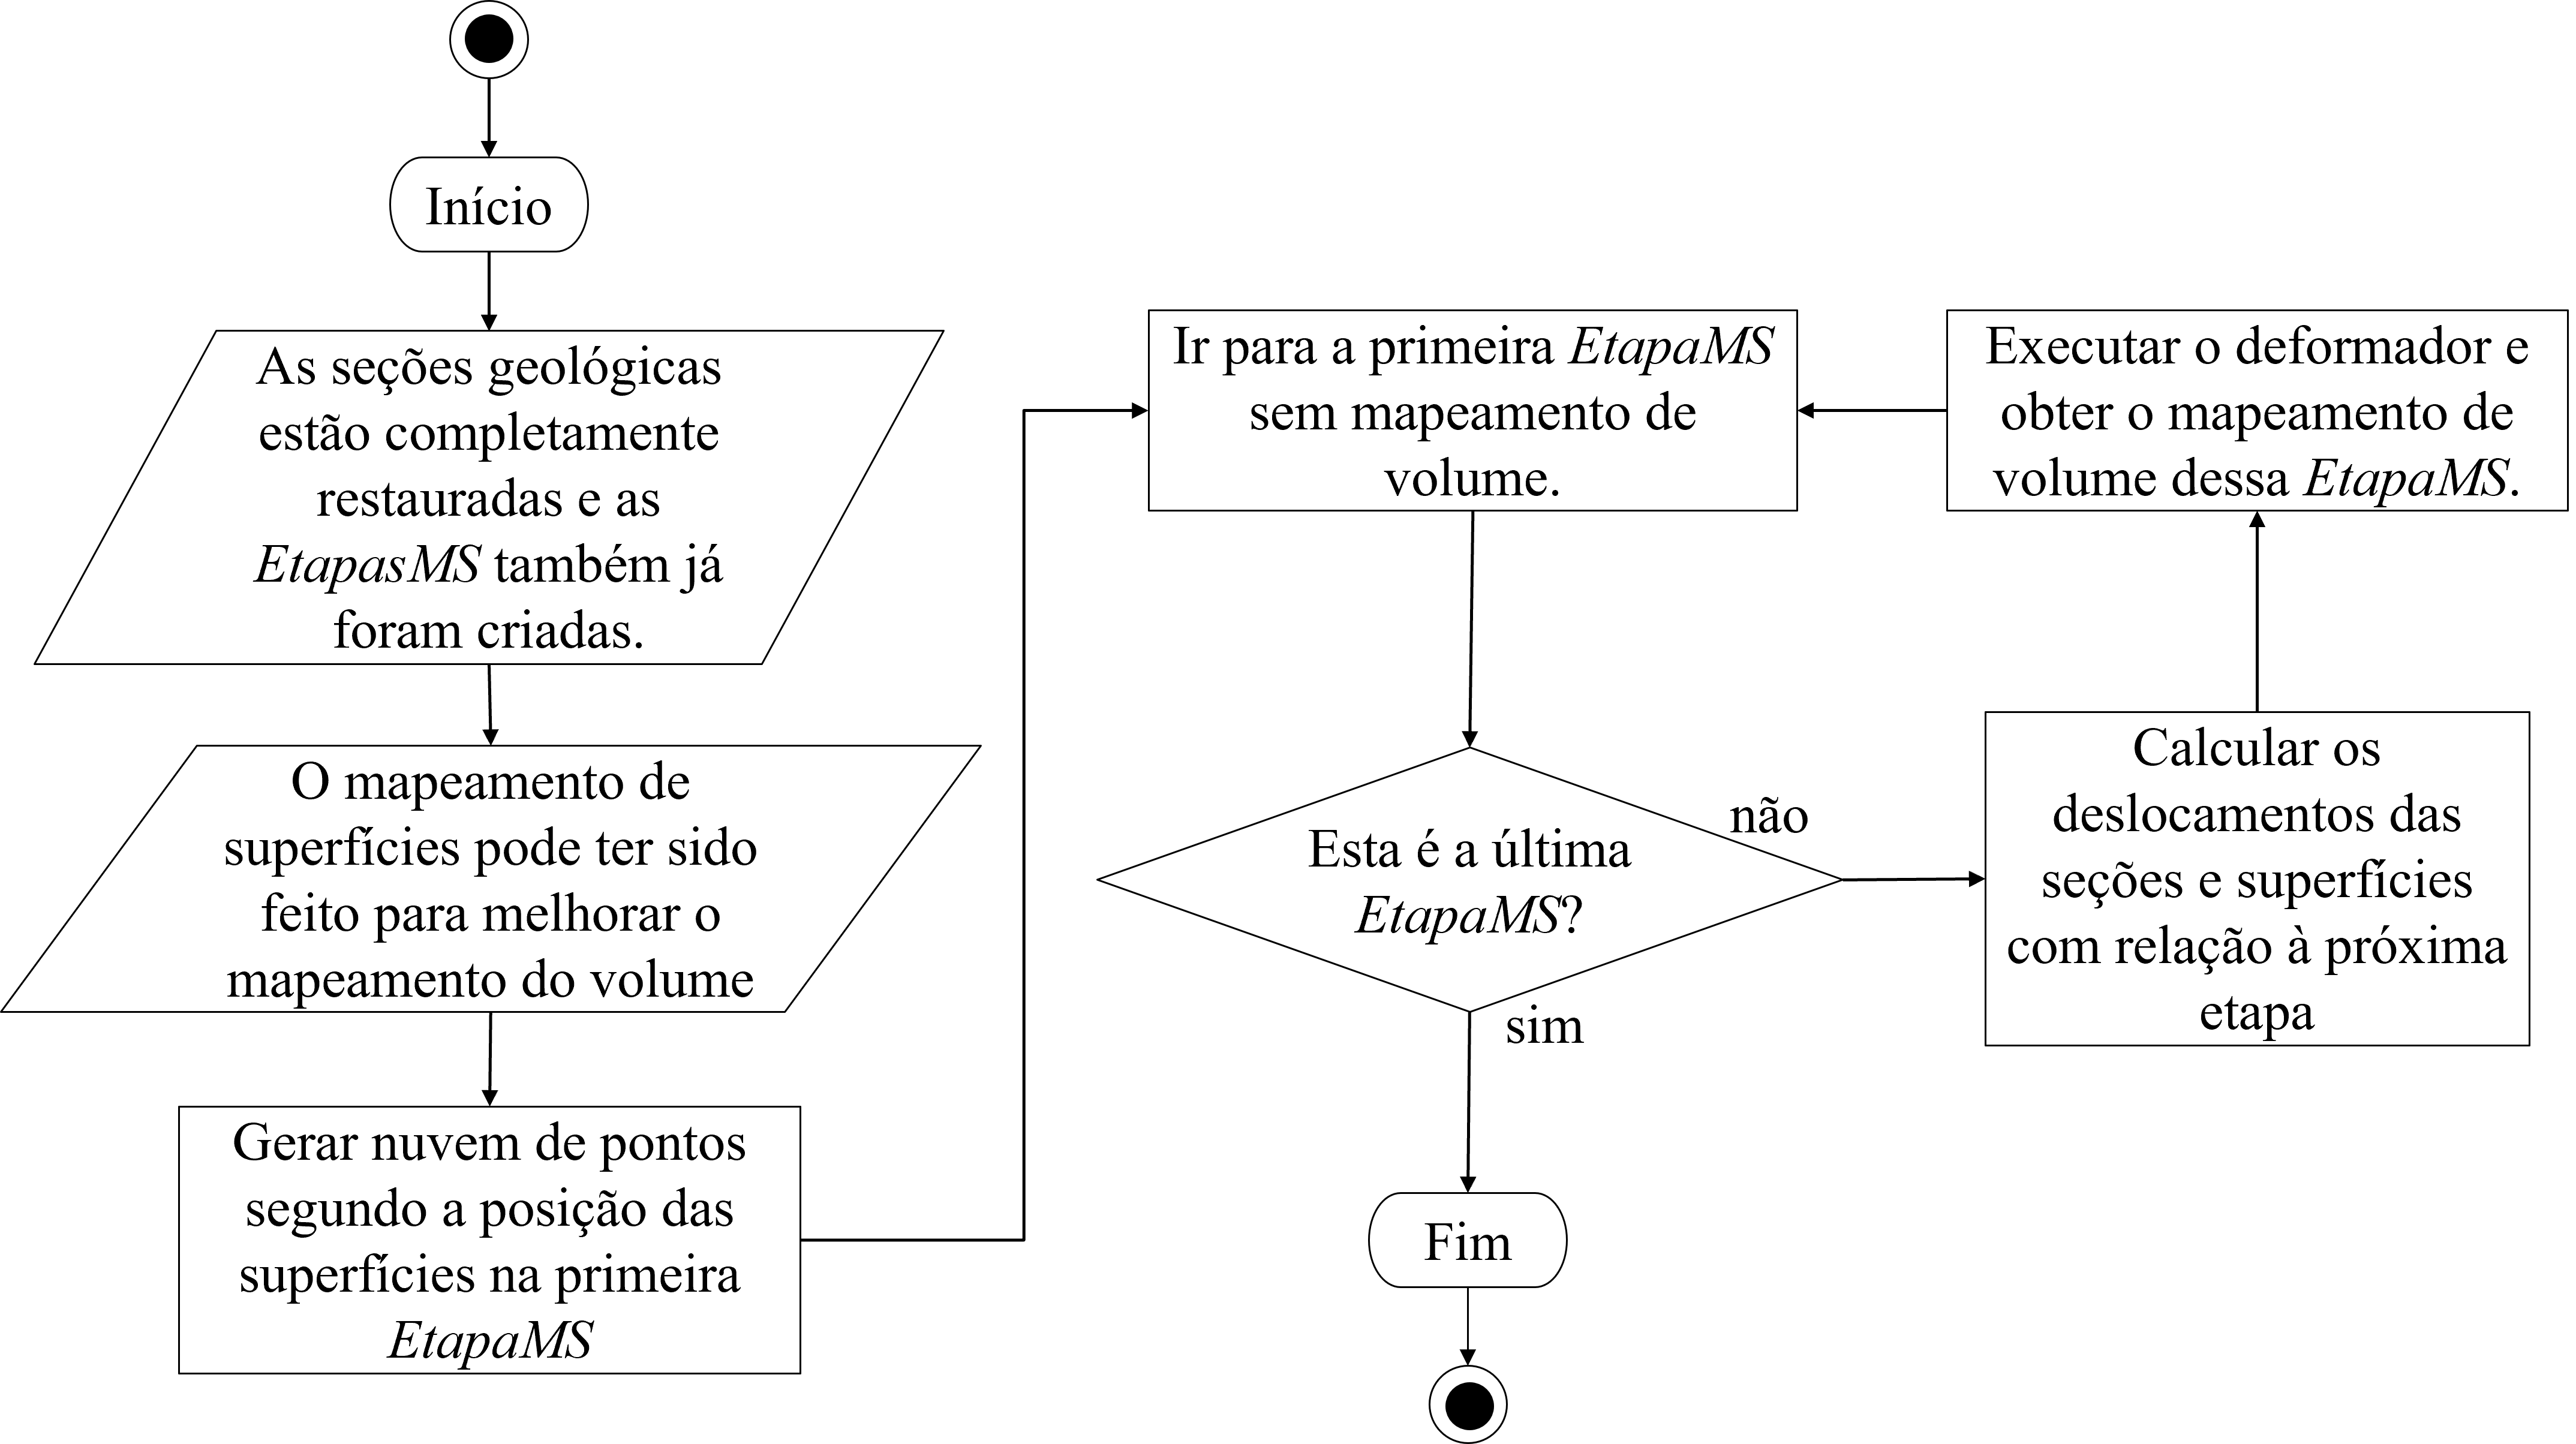
\includegraphics[width=\textwidth]{images/fig-volume-mapping-workflow}
    \caption{Fluxo de trabalho para executar o mapeamento do volume.}\label{fig-volume-mapping-workflow}
  \end{center}
\end{figure}

\subsection{Lista de falhas e \emph{EtapasMS}}

Assim como no mapeamento de superfícies, é preciso que o modelo esteja com a restauração das seções já finalizadas com \emph{EtapasMS} também prontas. Além disso, caso tenha sido feito o mapeamento de superfícies, é possível extrair dados desse mapeamento e assim ter ainda mais pontos contribuindo para a movimentação do volume\footnote{É possível realizar o mapeamento de superfícies em paralelo com o volume, bastando realizar a cada passo um e outro alternadamente.}.

Ao iniciar o mapeamento de volume, o primeiro passo é o levantamento de quantas \emph{EtapasMS} existem no modelo. Isso é necessário porque o mapeamento do volume também é feito por \emph{EtapaMS}, mais precisamente de uma \emph{EtapaMS} atual em relação à próxima. Ou seja, a entrada de dados vem principalmente das seções e superfícies em relação ao passo seguinte da restauração do modelo.

Após isso, busca-se todas as superfícies tridimensionais do modelo, incluindo as de falhas e horizontes. As superfícies são o principal parâmetro para a geração da nuvem de pontos que representam o volume discretizado\footnote{Para a geração da nuvem de pontos, as superfícies de horizonte precisam estar no estado original do modelo, ou seja, antes de haver deformação pelo mapeamento de superfícies. Nesse caso, são as superfícies da \emph{EtapaMS} inicial.}.

Com todos esses dados levantados, parte-se à geração da nuvem de pontos. Importante ressaltar que a geração da nuvem de pontos só é realizada uma única vez. Na etapa de descompactação serão removidos os pontos correspondentes à camada removida.

\subsection{Geração da nuvem de pontos}\label{cloud-points-generation}

A nuvem de pontos espaciais neste mapeamento, como já dito, é o volume geológico discretizado. Para sua criação, é preciso identificar o domínio tridimensional do modelo. Isto é feito com o cálculo da caixa envoltória de todo o modelo, em termos práticos, é a união das caixas envoltórias de todas as superfícies.

Com esta informação já é possível realizar a geração da grade volumétrica (Figura~\ref{fig-vol-grid}). Essa grade não é visualizada no modelo, apenas uma abstração utilizada no cálculo da movimentação e também para a geração dos pontos. Cada célula da grade é responsável por abrigar 8 pontos, como mostra a Figura~\ref{fig-vol-cell}.

\begin{figure} [H]
  \begin{center}
    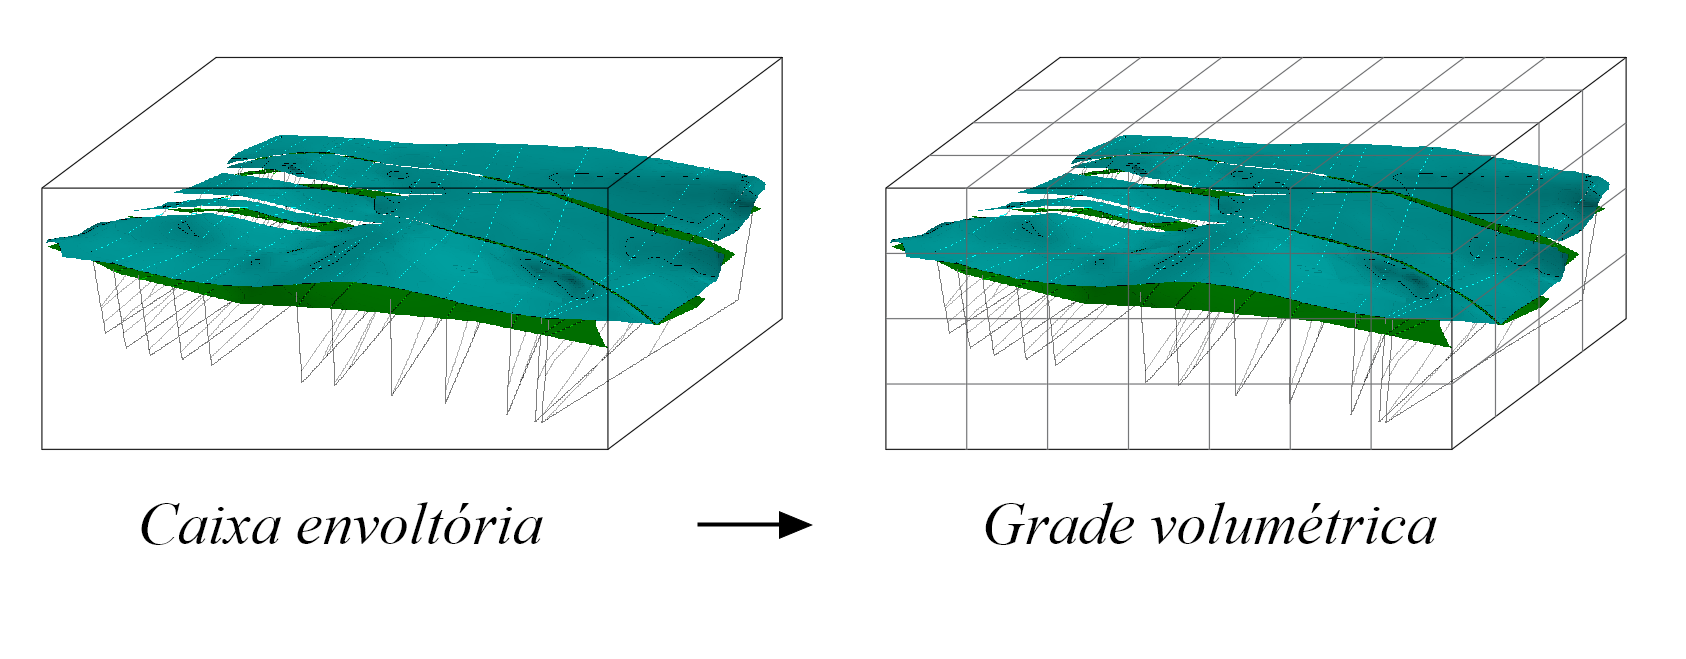
\includegraphics[width=\textwidth]{images/fig-vol-grid}
    \caption{Caixa envoltória e grade volumétrica do modelo geológico.}\label{fig-vol-grid}
  \end{center}
\end{figure}

\begin{figure} [H]
  \begin{center}
    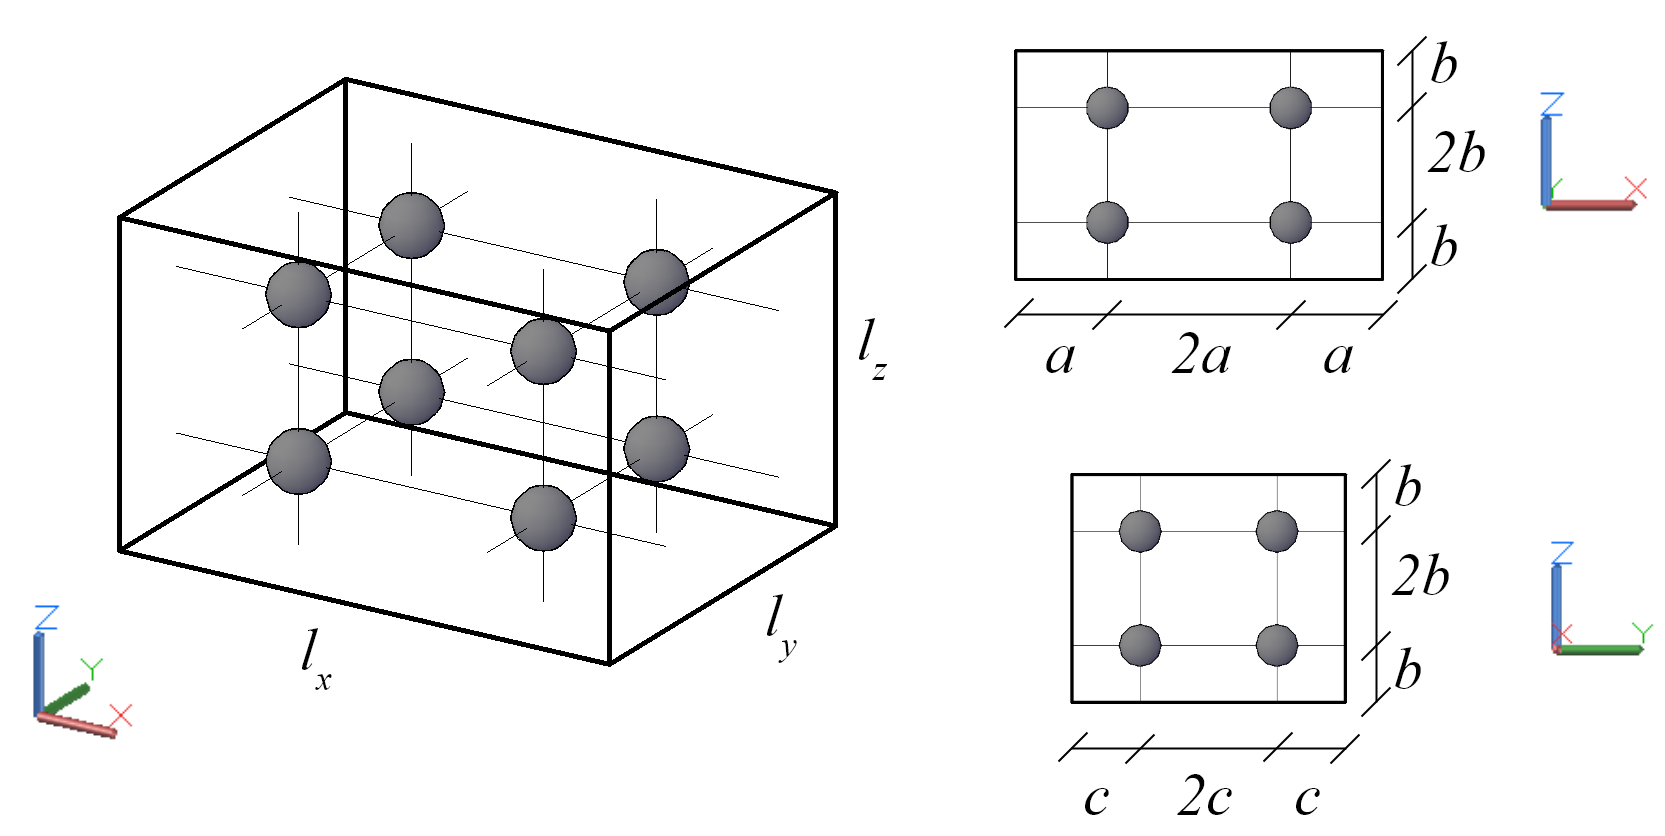
\includegraphics[width=\textwidth]{images/fig-vol-cell}
    \caption{Esquema de representação dos pontos em uma célula da grade.}\label{fig-vol-cell}
  \end{center}
\end{figure}

Cada célula possui as mesmas dimensões, na Figura~\ref{fig-vol-cell}, os comprimentos em $x$, $y$ e $z$ são obtidos pela divisão da caixa envoltória pelo número de subdivisões requerida e representados por $l_x$, $l_y$ e $l_z$ respectivamente. Os pontos internos são localizados segundo esses comprimentos; também na Figura~\ref{fig-vol-cell} as coordenadas são obtidas a partir de $a$, $b$ e $c$, que são, respectivamente, $l_x/4$, $l_z/4$ e $l_y/4$.

No entanto, apenas criar as células e então os pontos não é a única etapa. Os pontos que estão dentro da caixa envoltória mas fora do modelo geológico, precisam ser descartados. Ou seja, pontos acima da superfície de horizonte mais recente, precisam ser removidos. Além disso, dentre aqueles que restam é preciso que se defina a qual camada tal ponto pertence. Esta definição pode ser melhor explicada com uma ilustração em 2D, como na Figura~\ref{fig-vol-2d}. Cada ponto entre duas superfícies de horizonte é marcado como pertencente à camada de cima. Os pontos abaixo da última superfície (mais antiga) são definidos como pertencentes a esta.

\begin{figure} [H]
  \begin{center}
    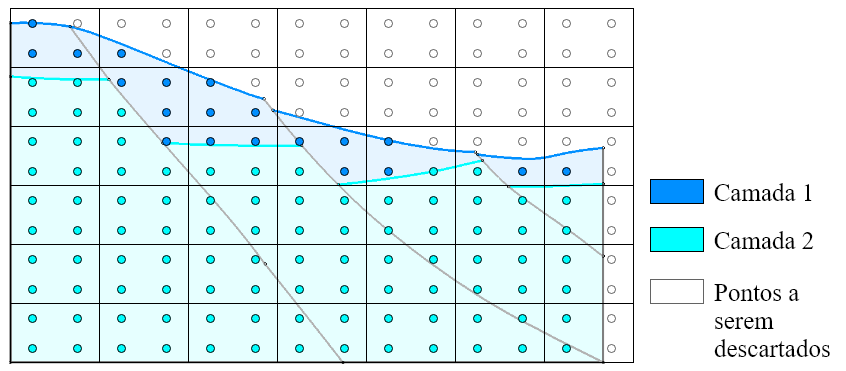
\includegraphics[width=\textwidth]{images/fig-vol-2d}
    \caption{Esquema de representação dos pontos em uma célula da grade.}\label{fig-vol-2d}
  \end{center}
\end{figure}

Para calcular, a cada ponto, se está abaixo ou acima de uma determinada superfície, é feito uma projeção no eixo $z$ do ponto de interesse nas superfícies e a partir do resultado, são avaliadas a qual camada pertence, conforme já explicado. Nesta projeção, é feito uma busca a partir do ponto da interesse para identificar quais os elementos da superfície mais próximos a ele e então realizar a projeção. A busca é feita com o auxílio de uma estrutura de dados \emph{R-tree}~\cite{RTree} criada a partir da malha da superfície.

Apesar de todos esses recursos para se gerar os pontos, descartar os de fora do domínio e ainda marcar a qual camada ele pertence, dependendo do modelo, podem haver pontos inconsistentes ou com marcação de camada errada. Isso pode acontecer quando a superfície apresenta buracos e, portanto, naquela região não terá uma projeção em $z$ existente, com isso, o ponto recebe a marcação da superfície de baixo, incorretamente, o que faz a nuvem de pontos apresentar unidades erroneamente. Casos assim são mostrados na Figura~\ref{fig-vol-errors}.

\begin{figure} [H]
  \begin{center}
    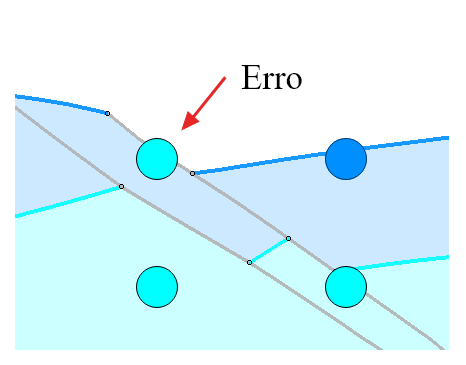
\includegraphics[width=200pt]{images/fig-vol-errors}
    \caption{Erro passível de ocorrer na geração da nuvem de pontos.}\label{fig-vol-errors}
  \end{center}
\end{figure}

Entretanto, são casos muito isolados e tendem a se reduzir ainda mais conforme se aumente o número de células na grade volumétrica. Além do mais, são problemas que não interferem na movimentação dos pontos. É algo que deixa a nuvem de pontos menos fidedigna ao volume geológico mas nem um pouco crítico.

\subsection{Movimentação dos pontos}

Com a nuvem de pontos já criada, pode-se iniciar a movimentação desses pontos segundo o deslocamento apresentado pelas seções e superfícies entre uma \emph{EtapaMS} e outra. 

Como já dito, uma \emph{EtapaMS} é um conjunto de cenários, cada um pertencente a uma seção. Pela \emph{EtapaMS} seguinte também é possível fazer a ligação entre um cenário e outro de uma seção. Mais especificamente, pela lista de \emph{EtapasMS} pode-se ter o histórico de cenários da restauração de uma seção.

O objetivo neste passo é ter o deslocamento dos pontos das malhas da seção entre uma \emph{EtapaMS} e a próxima. Este cálculo é feito semelhantemente à interpolação das \emph{LMModels} apresentada no item~\ref{lmmodels-surface-map}. Dessa forma, para cada ponto de malha da seção na \emph{EtapaMS} $A$ vai possuir um correspondente na malha da seção na \emph{EtapaMS} $B$.

Estes pontos são colocados em uma estrutura de dados especial e cada um com um atributo armazenando o seu destino na \emph{EtapaMS} seguinte.

O mesmo é feito para as superfícies após o mapeamento delas, com a vantagem de não precisar de uma interpolação (já que a malha da superfície não muda de uma \emph{EtapaMS} a outra). Para cada ponto da malha de superfície, é registrado seu correspondente na \emph{EtapaMS} seguinte. Os pontos das superfícies são adicionados à mesma estrutura de dados dos pontos das seções.

O último dado depende do tipo de marco geológico ocorrido entre as \emph{EtapaMS}. Em caso de descompactação, só são levados em conta pontos de seções e superfícies excluindo aqueles da camada a ser removida. Já em caso de restauração de falha, é preciso pegar os nós da malha da falha que está sendo restaurada e enviar ao deformador de volume como restrição junto da estrutura de dados com os pontos das seções e superfícies. Um resumo destes passos é apresentado na Figura~\ref{fig-vol-algorithm}.

\begin{figure} [H]
  \begin{center}
    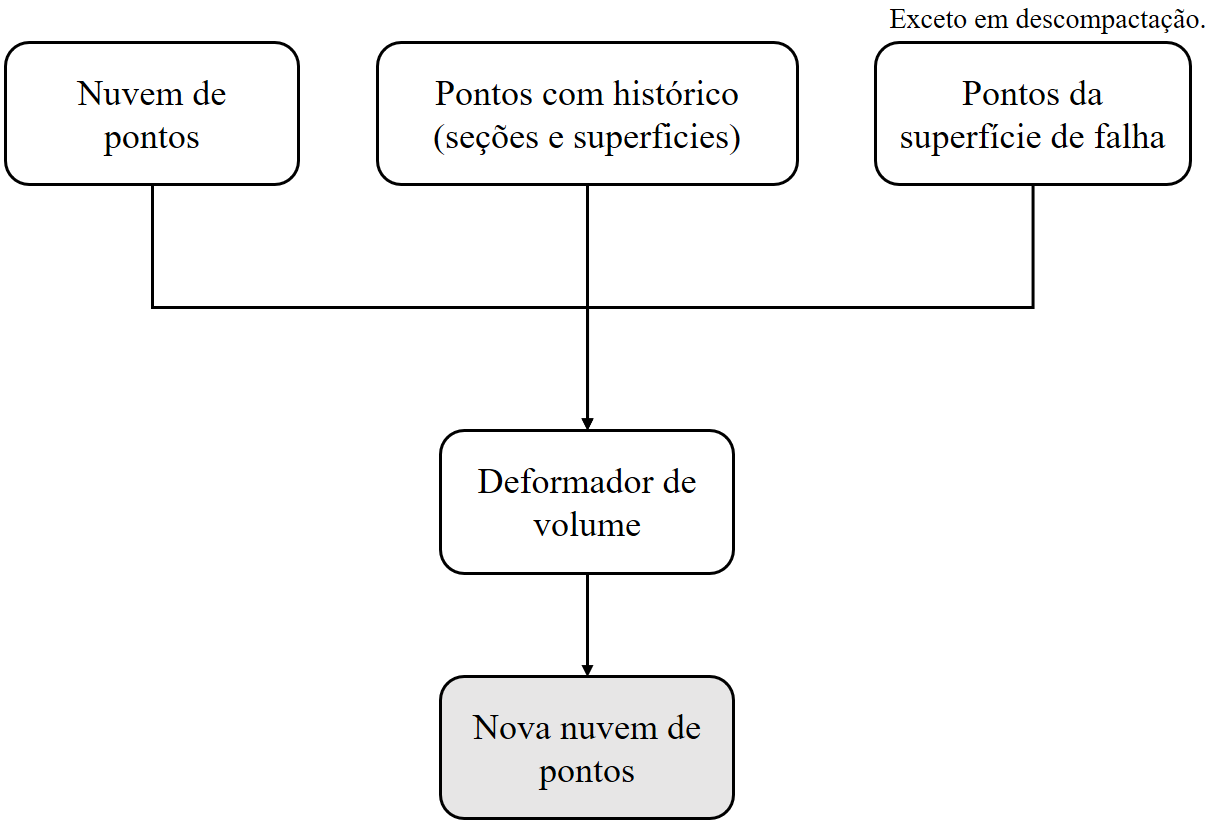
\includegraphics[width=350pt]{images/fig-vol-algorithm}
    \caption{Conjunto de dados para se fazer o mapeamento de volume.}\label{fig-vol-algorithm}
  \end{center}
\end{figure}

O resultado é uma nuvem de pontos atualizada que será usada no próximo passo do mapeamento e assim ter um volume coerente com o a movimentação tectônica das seções e superfícies.

\section{Exemplos e resultados}

Nesta seção é mostrado um exemplo de mapeamento do volume feito no mesmo modelo usado no mapeamento de superfície já apresentado no item~\ref{ex-2-surf}.

Para este exemplo foi adotada uma subdivisão para geração da grade volumétrica de $70$ unidades em $x$, $70$ unidades em $y$ e $60$ em $z$. Um total de $1.518.053$ pontos foram criados no domínio do modelo geológico\footnote{Ao realizar uma verificação simples, foram definidas $70\times70\times60=294.000$ células, cada uma contendo $8$ pontos, logo, aproximadamente $35\%$ dos pontos foram descartados por estarem fora do domínio do modelo.}. A Figura~\ref{fig-vol-ex-1} a seguir exibe o modelo geológico com apenas as superfícies de horizonte à esquerda e a nuvem de pontos gerada à direita.

\begin{figure} [H]
  \begin{center}
    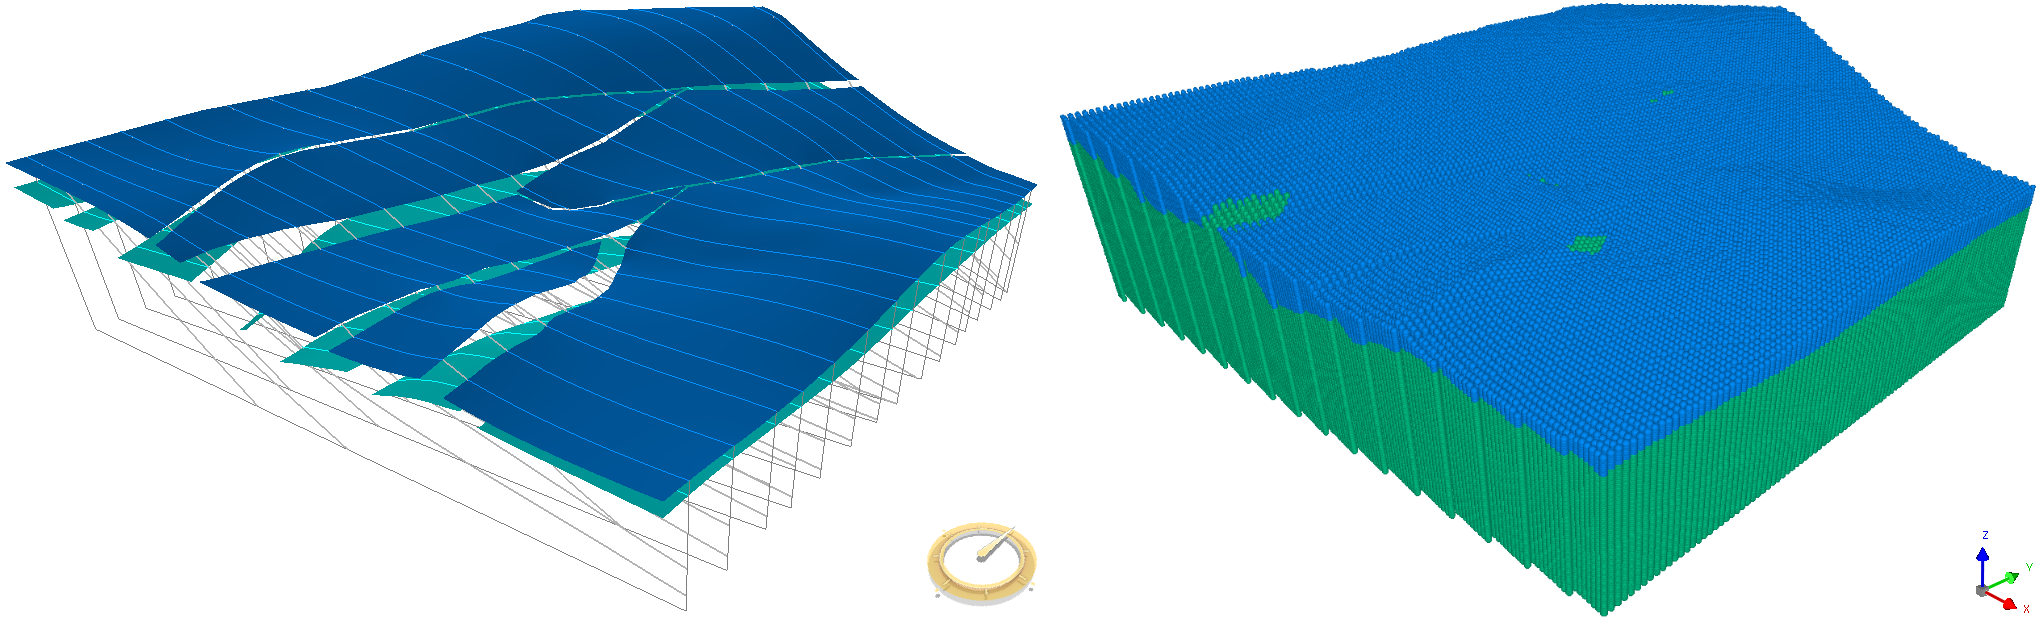
\includegraphics[width=\textwidth]{images/fig-vol-ex-1}
    \caption{Superfícies do modelo geológico e nuvem de pontos gerada.}\label{fig-vol-ex-1}
  \end{center}
\end{figure}

Observa-se na imagem da direita da Figura~\ref{fig-vol-ex-1} que há pontos no topo marcados como sendo da camada geológica de baixo, isso acontece pela presença de buracos na superfície do topo, problema discutido na seção~\ref{cloud-points-generation} (Figura~\ref{fig-vol-errors}).

Neste modelo já estão feitas todas as restaurações de seções e também o mapeamento de superfície (como apresentado na seção~\ref{ex-2-surf}). A primeira \emph{EtapaMS} restaura a falha 7 do modelo. Essa falha intercepta apenas 6 seções geológicas (Figura~\ref{fig-example-2-5}), logo apenas estas seções irão contribuir com pontos, cujos deslocamentos são maiores que zero, para a movimentação do volume. 

De acordo com o apresentado anteriormente, os pontos das seções e das superfícies são unidos numa estrutura de dados onde cada ponto possui um atributo guardando sua posição final na \emph{EtapaMS} seguinte. A Figura~\ref{fig-vol-ex-2} mostra os pontos dessa estrutura para esse primeiro passo, evidenciando apenas aqueles próximo das seções cruzadas pela falha 7, além dos pontos da própria superfície de falha 7.

Conforme metodologia apresentada (seção~\ref{vol-metodology}), a movimentação conhecida dos pontos de seção e superfície é a responsável por fazer a movimentação dos pontos do volume. Para esta \emph{EtapaMS} é apresentada na Figura~\ref{fig-vol-ex-3} a nova nuvem de pontos com a execução do deformador de volume.

\begin{figure} [H]
  \begin{center}
    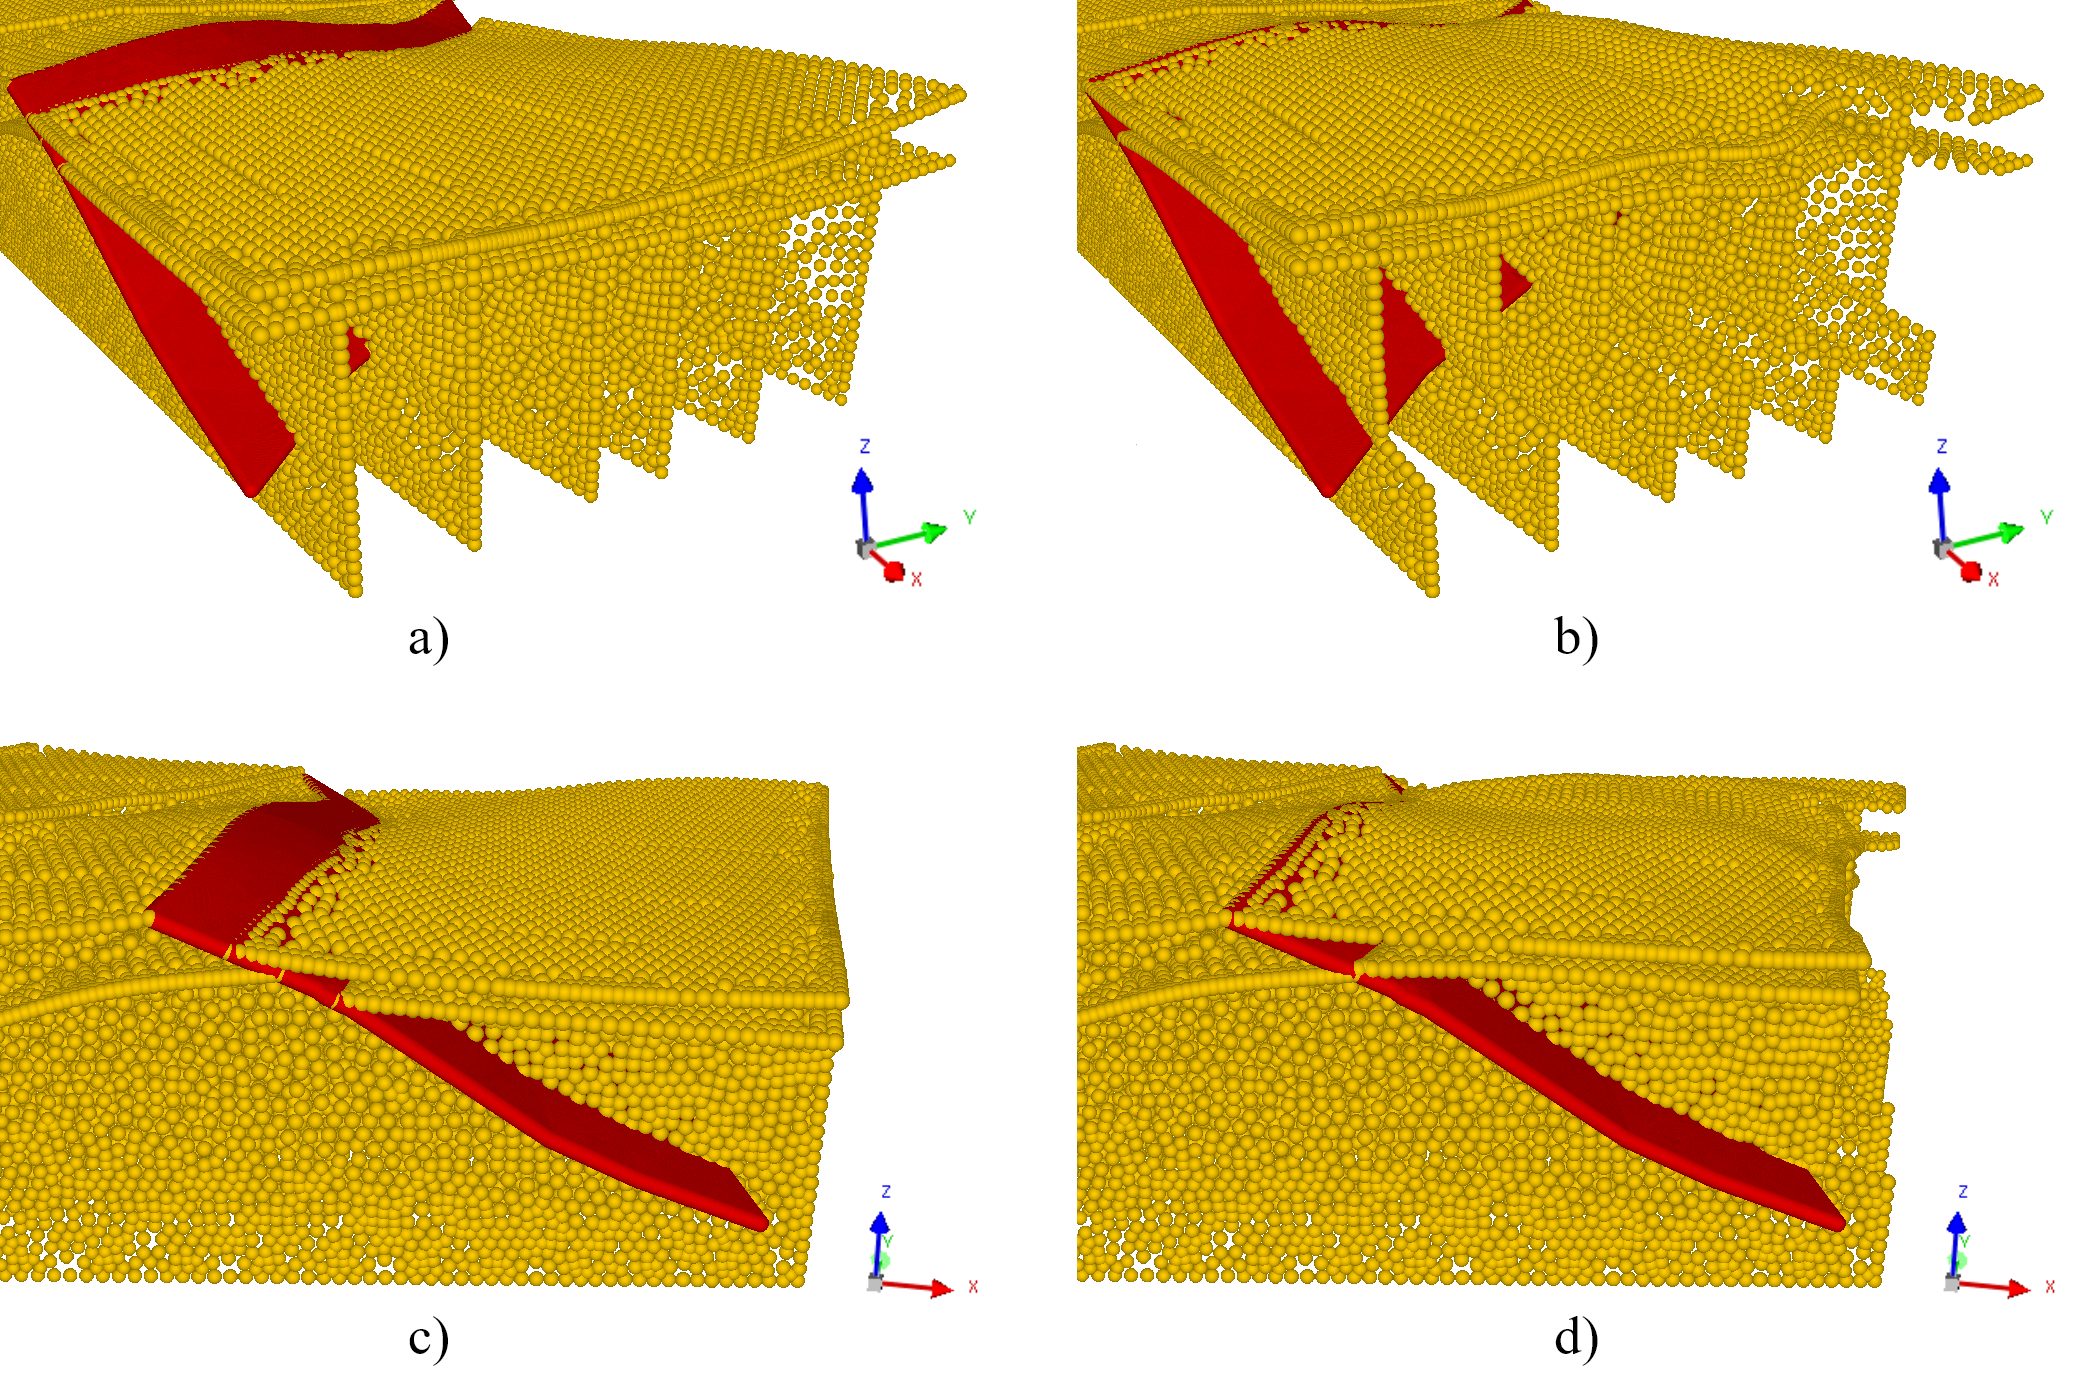
\includegraphics[width=\textwidth]{images/fig-vol-ex-2}
    \caption{Pontos com informação de movimentação da primeira etapa do mapeamento do volume: (a) e (c) antes do movimento, (b) e (d) após o movimento.}\label{fig-vol-ex-2}
  \end{center}
\end{figure}

\begin{figure} [H]
  \begin{center}
    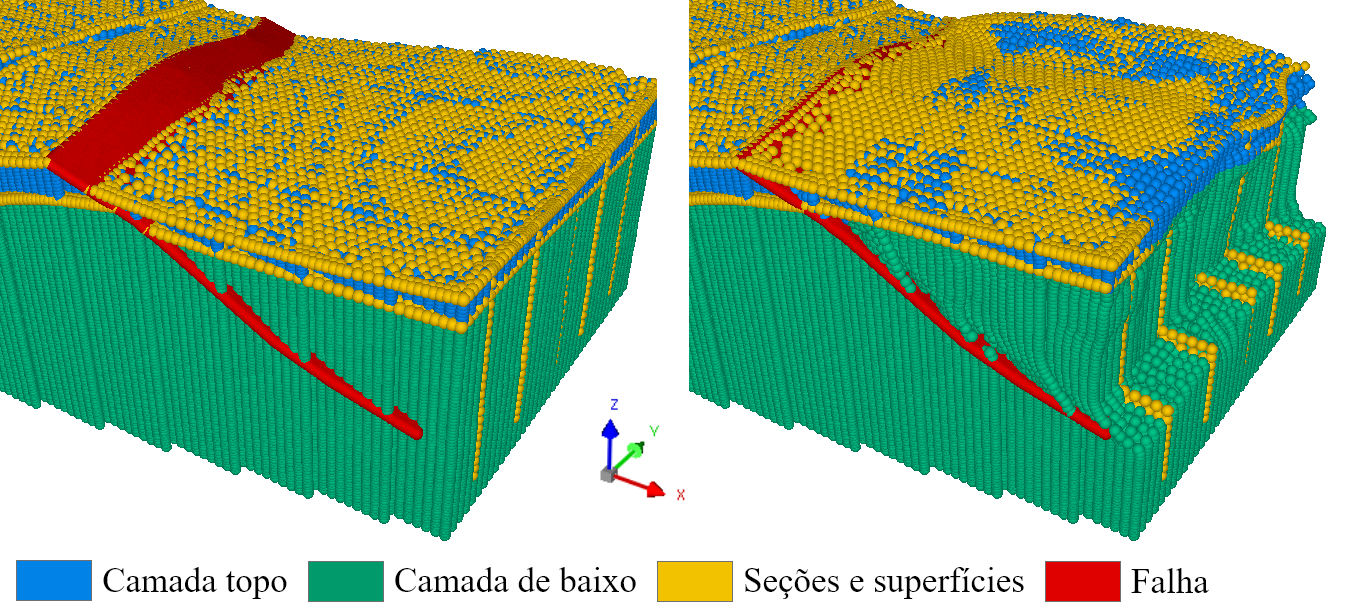
\includegraphics[width=\textwidth]{images/fig-vol-ex-3}
    \caption{Movimentação da nuvem de pontos devido à primeira \emph{EtapaMS} de restauração do modelo.}\label{fig-vol-ex-3}
  \end{center}
\end{figure}

Diferente do mapeamento de superfícies, aqui no volume não há necessidade de uma interação, só é preciso que os requisitos estejam prontos (seções e superfícies). Nas Figuras~\ref{fig-vol-ex-4} a~\ref{fig-vol-ex-7} são mostrados o mapeamento do volume para cada \emph{EtapaMS} subsequente até que se tenha a camada do topo restaurada.

\begin{figure} [H]
  \begin{center}
    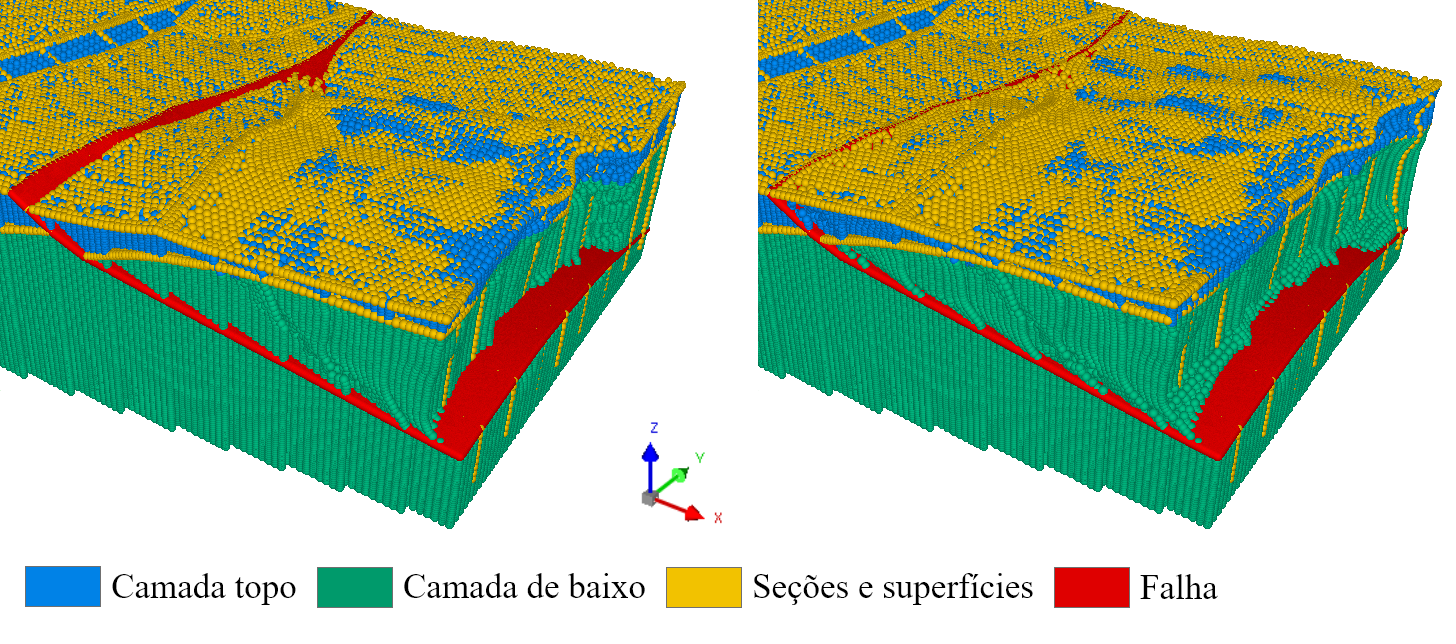
\includegraphics[width=\textwidth]{images/fig-vol-ex-4}
    \caption{Movimentação da nuvem de pontos devido à \emph{EtapaMS} que restaura a falha 6.}\label{fig-vol-ex-4}
  \end{center}
\end{figure}

\begin{figure} [H]
  \begin{center}
    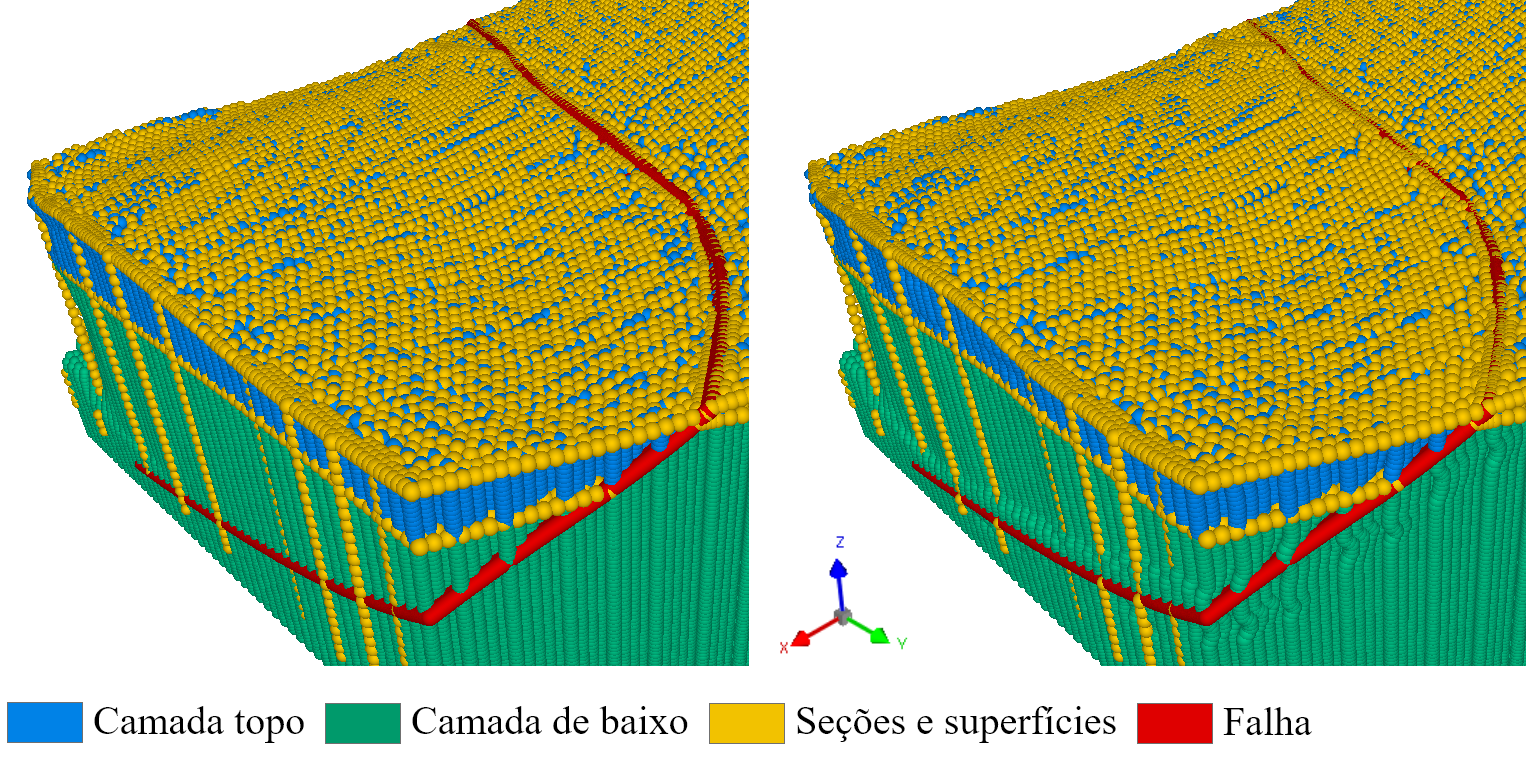
\includegraphics[width=\textwidth]{images/fig-vol-ex-5}
    \caption{Movimentação da nuvem de pontos devido à \emph{EtapaMS} que restaura a falha 5.}\label{fig-vol-ex-5}
  \end{center}
\end{figure}

\begin{figure} [H]
  \begin{center}
    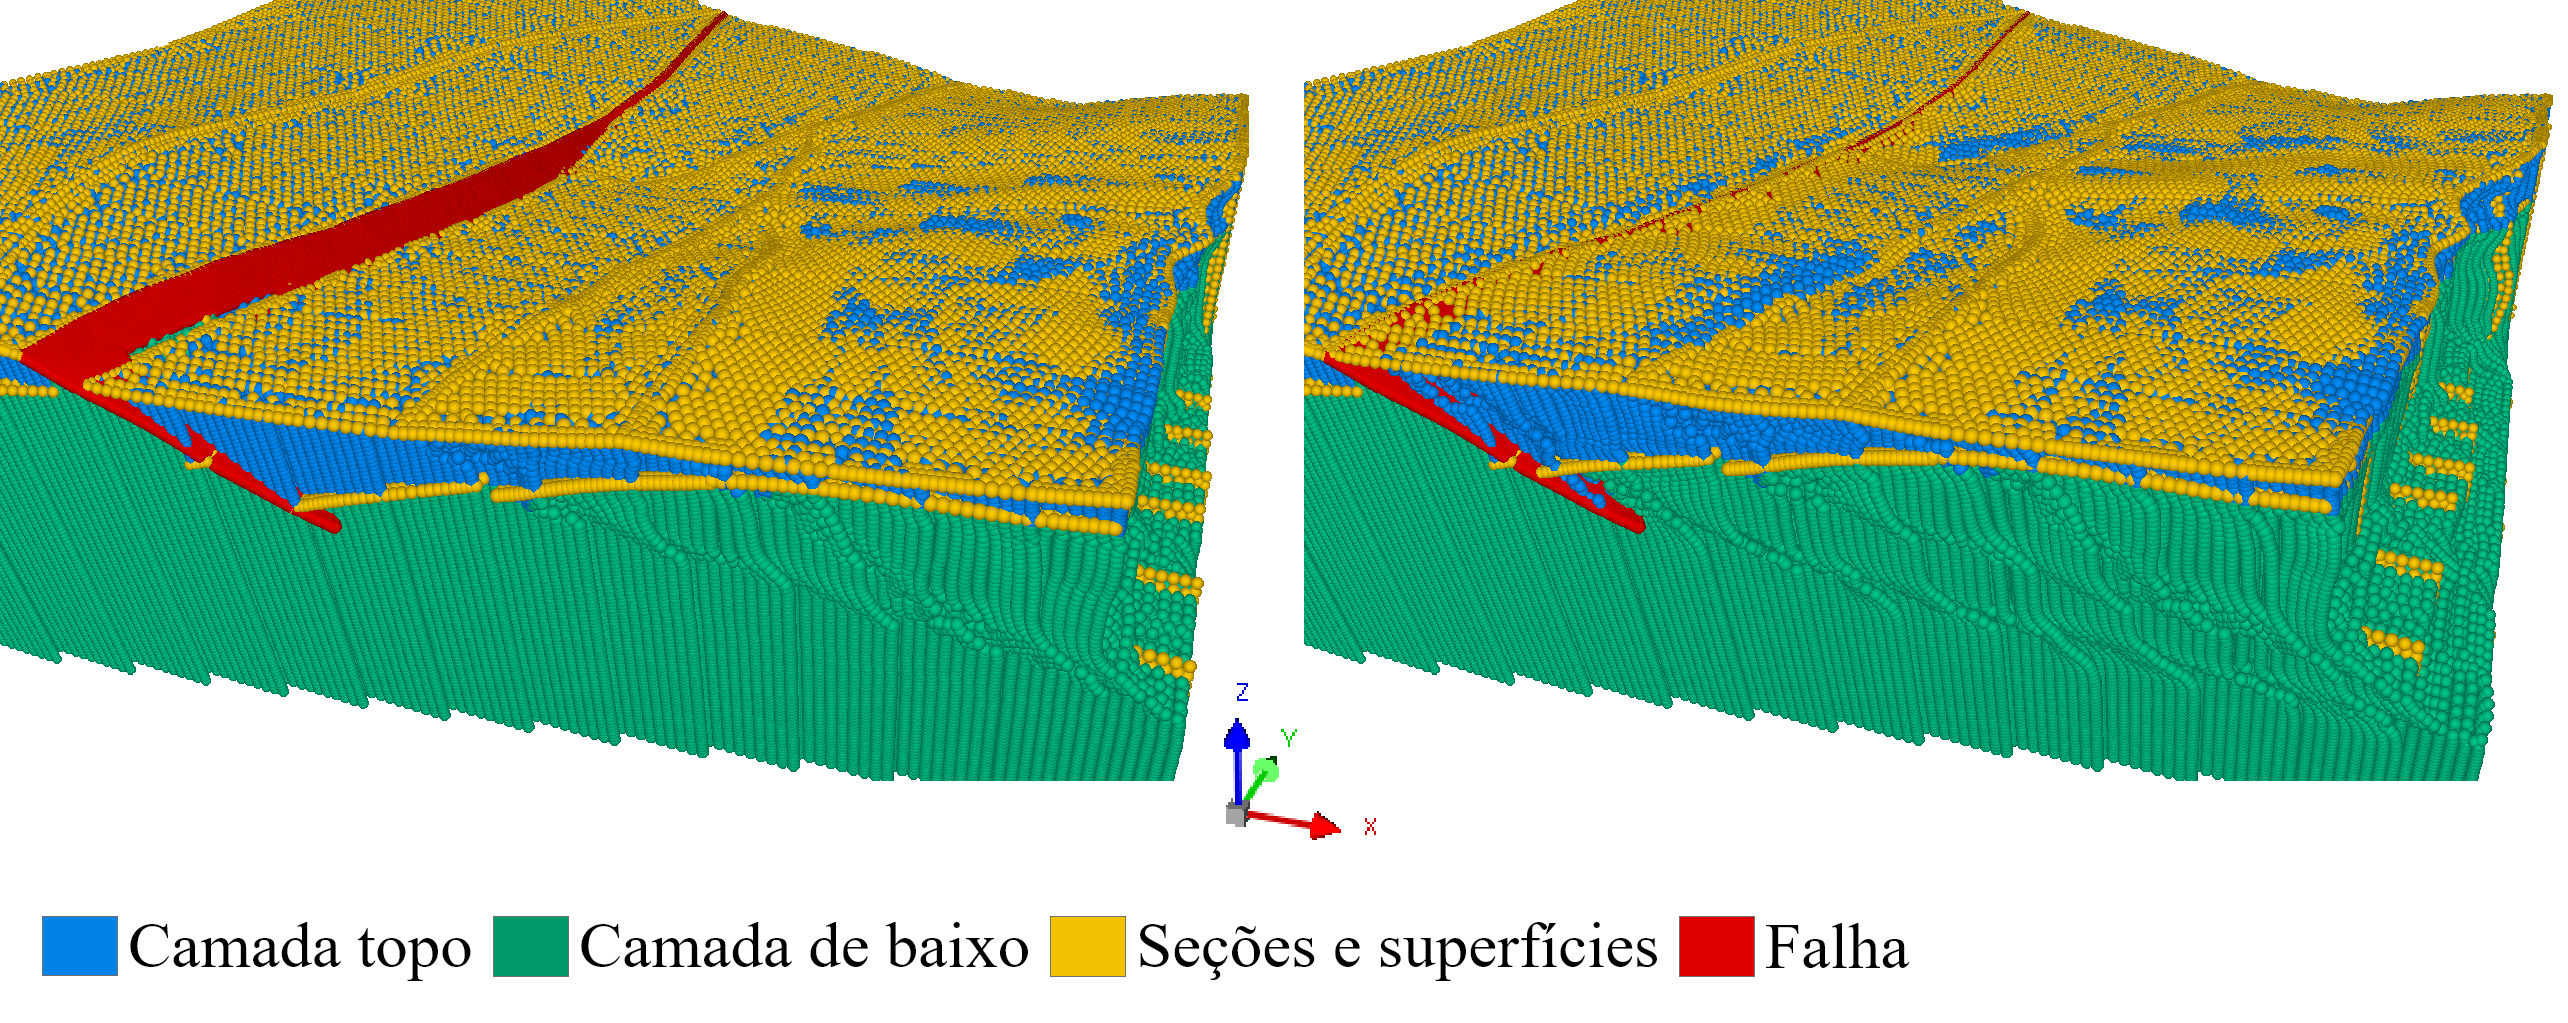
\includegraphics[width=\textwidth]{images/fig-vol-ex-6}
    \caption{Movimentação da nuvem de pontos devido à \emph{EtapaMS} que restaura a falha 4.}\label{fig-vol-ex-6}
  \end{center}
\end{figure}

\begin{figure} [H]
  \begin{center}
    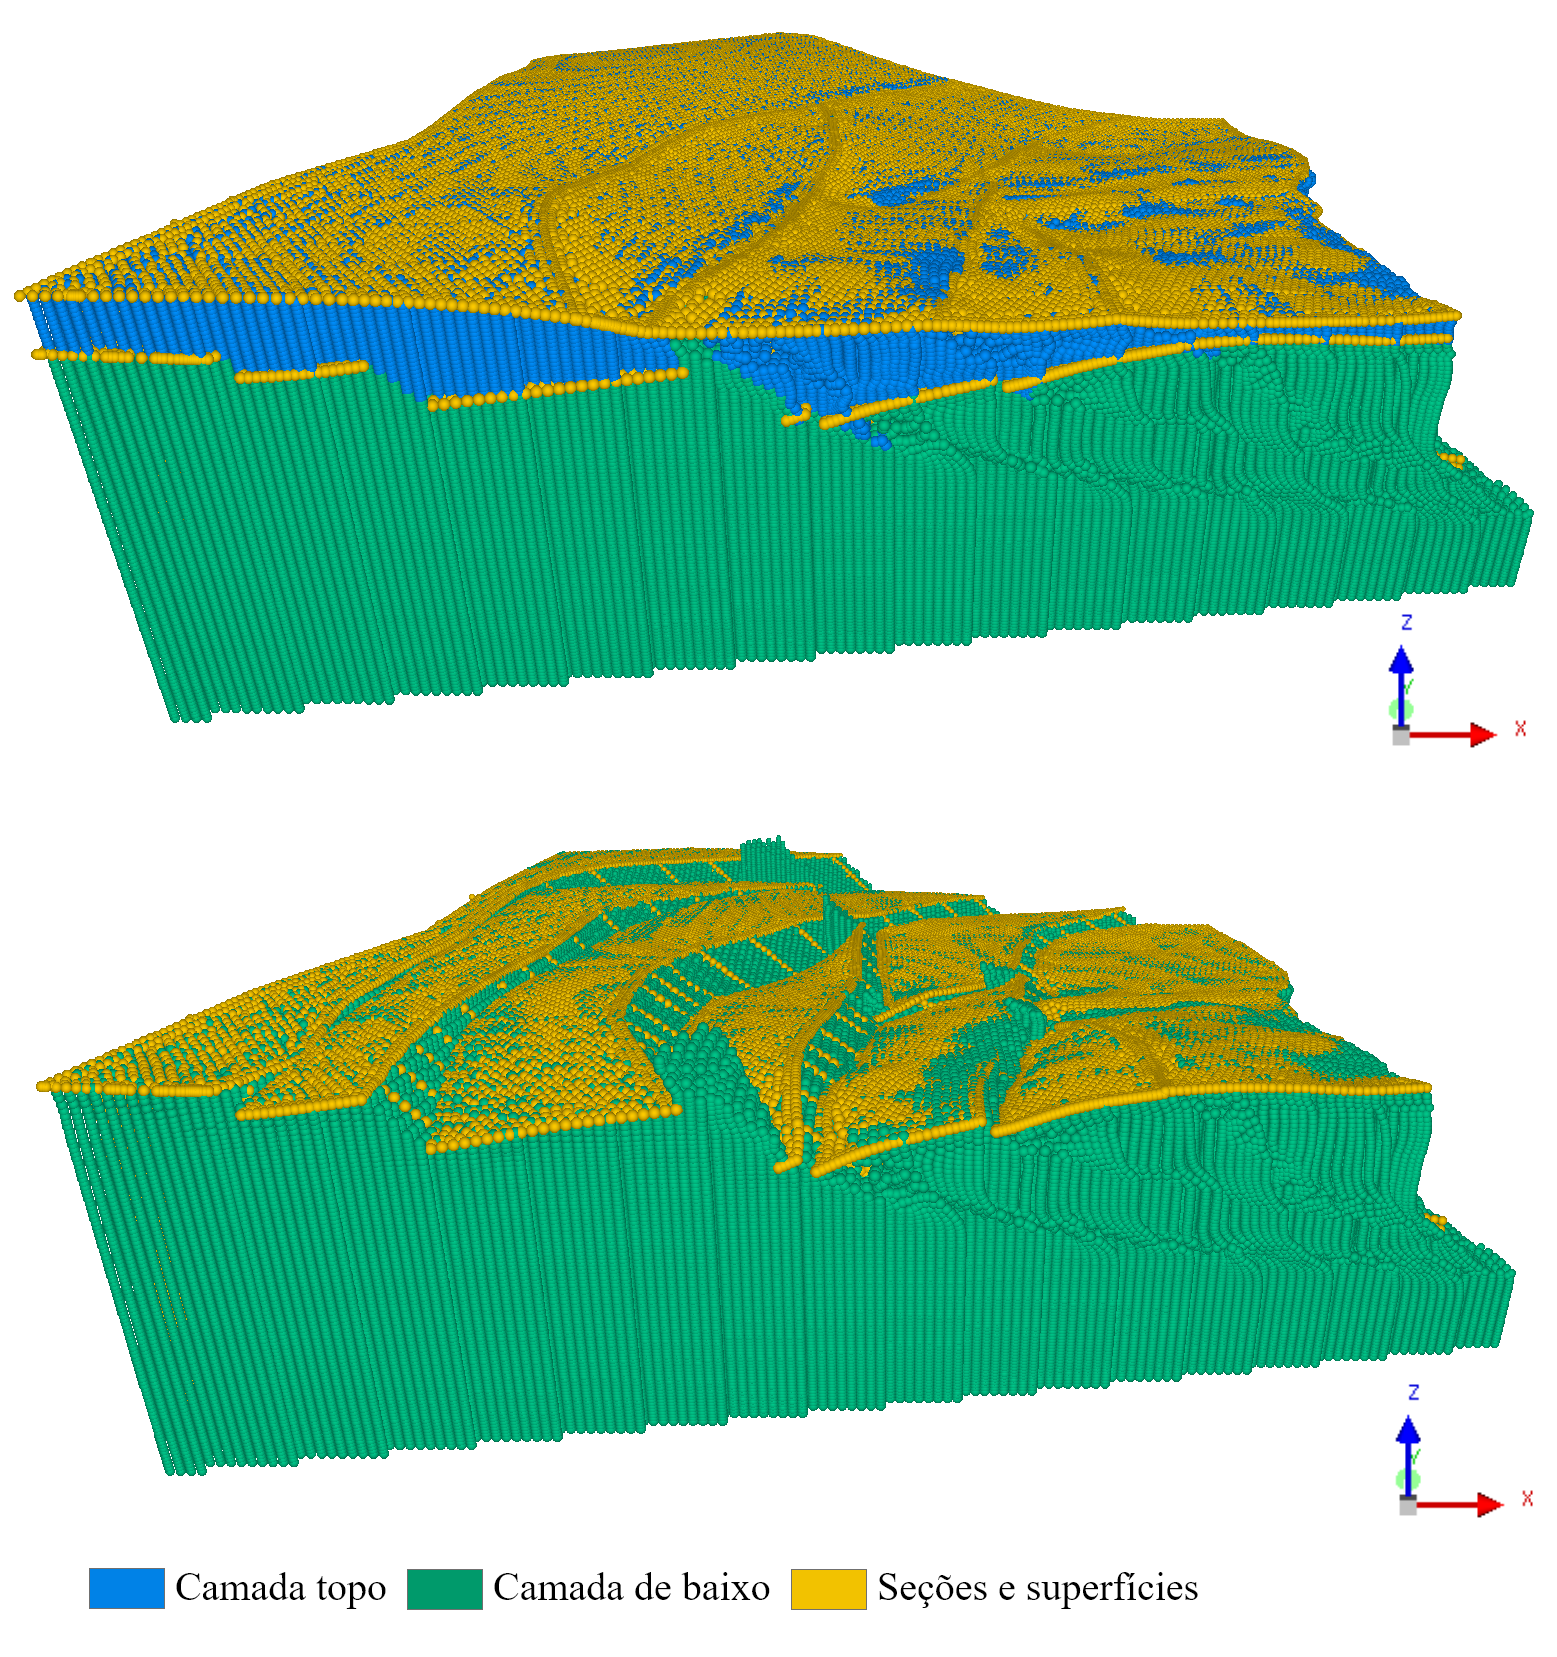
\includegraphics[width=350pt]{images/fig-vol-ex-7}
    \caption{Movimentação da nuvem de pontos devido à \emph{EtapaMS} de descompactação da camada do topo.}\label{fig-vol-ex-7}
  \end{center}
\end{figure}

Quando há uma \emph{EtapaMS} de descompactação, os pontos de seções e superfícies continuam sendo guia de movimentação porém, os pontos da camada do topo são removidas da nuvem de pontos e assim manter o volume do modelo atualizado segundo o estado corrente da restauração. A Figura~\ref{fig-vol-ex-7} mostra o antes e depois da descompactação neste modelo usado como exemplo.

Conforme os resultados obtidos, a movimentação do volume pode ser vista como uma boa aproximação em relação à restauração das seções, respeitando, inclusive, a restrição das superfícies de falhas.

Este processo de mapeamento do volume apresenta facilidade de uso e representa bem modelos geológicos complexos, sem uma necessidade explícita de definição desse volume. Além do mais, o método numérico empregado é capaz de fornecer bons resultados com eficiência computacional.

Com esta metodologia tem-se a possibilidade de mapear um ponto qualquer no ambiente multisseções ao longo da restauração de um modelo geológico. Há ainda a chance de movimentar pontos de seções não restauradas com base na restauração das demais, uma forma de restaurar uma seção geológica passivamente.
